\chapter{Создание набора данных} \label{cha:dataset}

На русском языке не существует набора данных, подходящего для целей исследования. 
Поэтому придётся создавать его самостоятельно.
Для этого потребуется определить два корпуса: первый, состоящий из текстов в формальном стиле, и второй, состоящий из текстов в неформальном стиле.
Затем, согласно главам \ref{cha:analysis:sec:target} и \ref{cha:analysis:sec:datasets}, для части предложений из неформального корпуса необходимо создать их формальные парафразы.

\section{Обзор наборов данных, подходящих для аннотации}
Можно определить доступные корпуса на русском языке: Википедия, новостные издания, литература, печатные издания, субтитры, социальные сети, специализированные наборы данных для конкретных задач (например, детоксификация текста).

Социальные сети на первый взгляд подходят для создания неформального корпуса, однако стилистические атрибуты в них крайне неоднородны и значительно различаются у разных пользователей. Так же большое количество пользователей использует достаточно нейтральный стиль в своих комментариях.

% Луркморе как антипод википедии. Стилестически выдержаный. Достаточный объём.
Интересным кандидатом для использования в качестве источника неформального текста является база статей сайта Луркморье\footnote{Оригинальный сайт удалён владельцем. Обновлённая версия: https://neolurk.org/wiki/Луркморье} (Lurkmore) за 2021 год.
Луркморье -- русскоязычная интернет-энциклопедия, аналог Википедии, функционирующая на том же движке MediaWiki, но написанная в неформальном стиле, изобилующая жаргонами и интернет-мемами, и позиционирующая себя как <<энциклопедия современной культуры>>.
Данный сайт, помимо того, что удовлетворяет критерию неформального стиля, является стилистическим антиподом Википедии.
Также база статей имеет достаточный объём (около 9 тысяч статей, состоящих из более 600 тысяч предложений различной длины) для использования в обучении современных нейросетевых алгоритмов.

В данной работе выбор был сделан в пользу пары Луркморье-Википедия. Главной причиной такого решения является жанровая близость двух этих корпусов (здесь под жанром подразумевается функциональная направленность текста, как в работе \textit{Functional Text Dimensions for annotation of Web corpora} \cite{sharov_corpora}). Тексты из обоих корпусов являются энциклопедическими статьями, информирующими читателя о объектах действительности и явлениях. 

Для разбивки текста на предложения был использован токенизатор Razdel от проекта Natasha\footnote{https://github.com/natasha/razdel}.
Затем принимались только предложения, соответствующие следующим параметрам:
\begin{itemize}
    \item длина от 80 символов
    \item минимум 5 слов в предложении
    \item обязательно должна присутствовать кирилица.
\end{itemize}
Из базы можно получить около 423 тысяч предложений, что соответствует 125 МБ текста.
Таким образом в итоговом корпусе оказалось 423974 предложения.


\section{Разметка данных}
\subsection{Толока}
Как было упомянуто в \ref{cha:analysis:sec:target} 10000 пар предложений формальный-неформальный стиль являются желаемым результатом. Такое в одиночку не сделать, поэтому необходимо воспользоваться помощью асессоров. И подходящим сервисом для решения этой задачи является сервис Толока\footnote{https://toloka.ai/} -- платформа для привлечения асессоров к разметке данных.

% Однако, следует обратить внимание на наборы данных, изначально собранных для похожих задач, а также на других языках. Потому что это лучше поможет понять задачу и убережёт от вероятных ошибок в создании собственного набора данных.
Основная сложностью в процессе привлечения сторонних людей является описание задания, написание инструкции и фильтр подходящих кандидатов \cite{dementieva2021crowdsourcing}.

% Тестовый запуск на 100 предложений. Описание запуска. Результаты. Ошибки толокеров. Дороговизна
Для проверки работоспособности подхода было принято решение запустить тестовое задание на 100 случайных предложений из выборки.
На рисунках \ref{fig:toloka_instruction_1} и \ref{fig:toloka_instruction_2} представлена инструкция, выдаваемая асессорам. 
В ней пользователю Толоки объясняется, что нужно перефразировать предложения из сленга в формальный стиль.
Даётся пример источников текста в формальном стиле.
Затем приводится несколько примеров перефразов.
В инструкции также указывается предупреждение, что в задании может содержаться оскорбительный контент.
Также толокеру сообщается, что неформальность заключается не только в наличии сленга, но и в стилистике предложения. Приведены несколько примеров.
Указывается, что в случае невозможности перевести предложение или в случае, если толокер считает его уже формальным, необходимо его пропустить

\begin{figure}[ht]
  \centering
   \frame{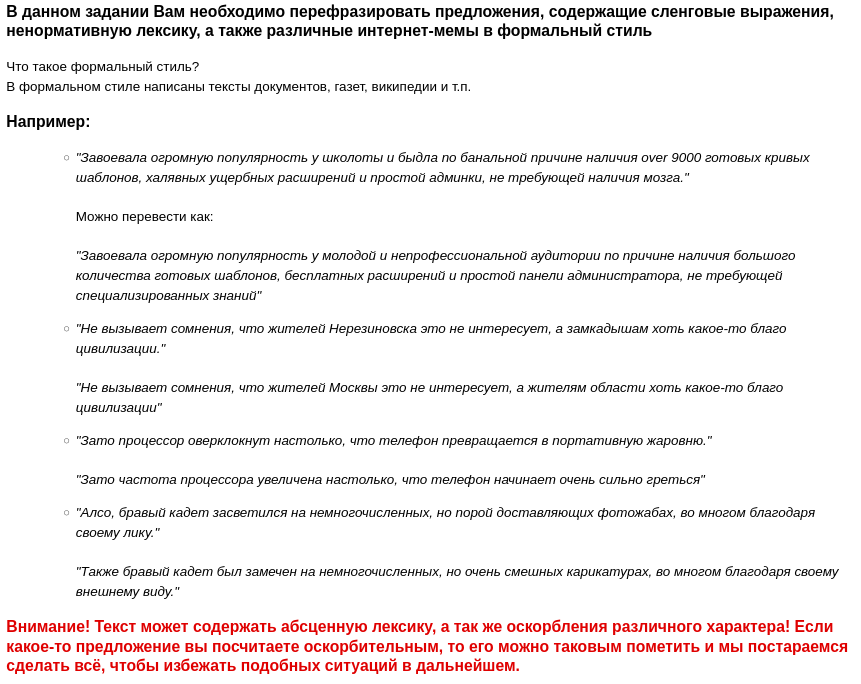
\includegraphics[width=\textwidth]{figures/toloka_instruction_1.png}}
  \caption{Первая часть инструкции для разметчиков}
  \label{fig:toloka_instruction_1}
\end{figure}

\begin{figure}[ht]
  \centering
  \frame{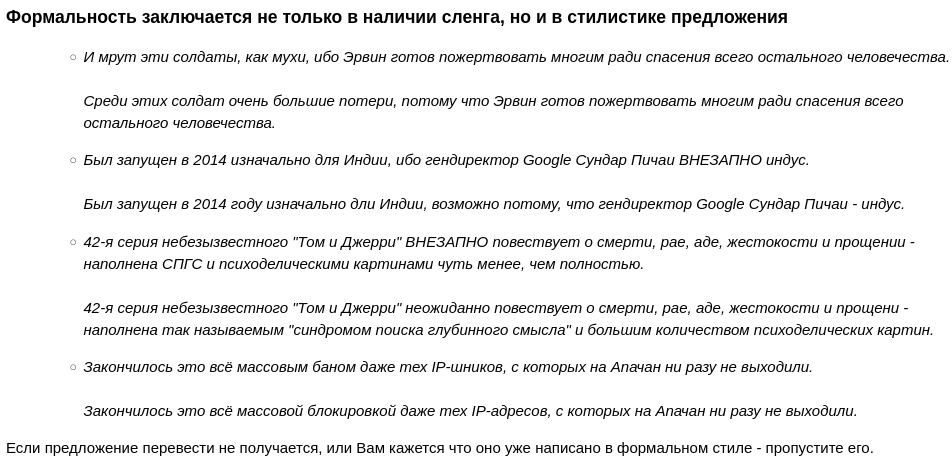
\includegraphics[width=\textwidth]{figures/toloka_instruction_2.png}}
  \caption{Вторая часть инструкции для разметчиков}
  \label{fig:toloka_instruction_2}
\end{figure}

Само задание представляет лишь обязательное поле, в которое асессор должен записать парафраз.
Изображение интерфейса задания представлено на рисунке \ref{fig:toloka_input_field}.
На одну страницу давалось одно задание, чтобы асессор мог на нём сфокусироваться. Временной лимит устанавливался в 10 минут.

\begin{figure}[ht]
  \centering
  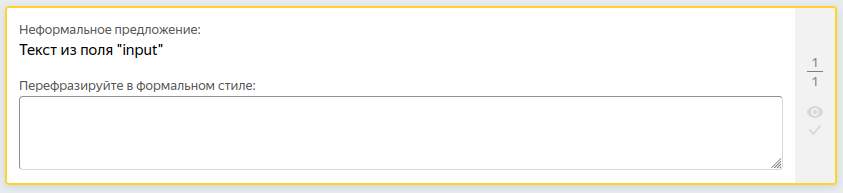
\includegraphics[width=\textwidth]{figures/toloka_input_field.png}
  \caption{Окно задания для разметчика}
  \label{fig:toloka_input_field}
\end{figure}

Так же было установлено тридцатипроцентное качество исполнителей. Установлено перекрытие равное 2, т.е. каждое предложение продублируется двум разным исполнителям.
И, самое главное, была установлена отложенная приёмка, что означает, что асессоры получат деньги, лишь при явном одобрении результата.
Полный список настроек представлен на рисунке \ref{fig:toloka_settings}.

\begin{figure}[ht]
  \centering
  \frame{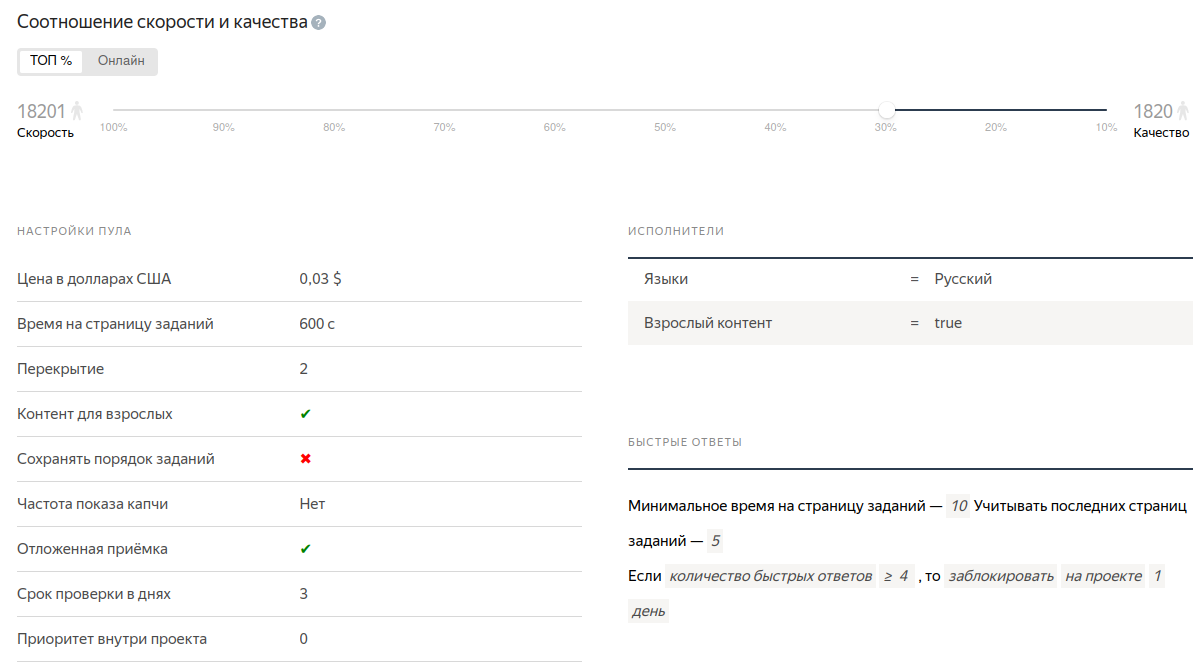
\includegraphics[width=\textwidth]{figures/toloka_settings.png}}
  \caption{Параметры задания}
  \label{fig:toloka_settings}
\end{figure}

Получились следующие результаты. Для 100 предложений с перекрытием 2 было создано 200 заданий. После ручной проверки были приняты 96 перефразов, 44 был отклонены и с 60 ответами возникли трудности. Постановку задачи можно считать удовлетворяющей.

Однако, у многих асессоров возникли некоторые трудности:
\begin{itemize}
    \item Грамматические ошибки. Исполнитель либо опечатался, либо использовал неправильно причастие или спряжение, таких случаев немного. Такие предложения можно принять, потому что эти ошибки можно легко выявить и исправить.

    \item Формализована лишь часть предложения. Распространённый случай, когда, например, исполнитель заменил обсценное слово на нейтральное, но в тоже время не затронул другие стилистически неформальные конструкции.

    \item Исполнитель не понял сленга. Здесь исполнитель либо не распознал отсылку на интернет-мем, либо неправильно её понял.

    \item Искажён смысл. Ошибка зачастую связанная с предыдущей, когда асесор очевидным образом изменил посыл предложения.

    \item Также распространены случаи, когда исполнитель вроде перефразировал, выполнил задачу, но стилистически текст всё ещё несёт в себе просторечия.
\end{itemize}

Сразу появилось много идей, как можно улучшить качество:
\begin{itemize}
    \item Добавить обучение
    \item Увеличить соотношение качество/скорость
    \item Увеличить перекрытие (затратно)
    \item Запускать разметку по частям и отфильтровывать исполнителей
    \item Расписать более подробно критерии приёмки
    \item Уменьшить длину предложений
\end{itemize}

Также необходимо оценить финансовые затраты.
В среднем асессор тратил около двух минут на выполнение задания (немного медленнее, чем в \cite{dementieva2021crowdsourcing}), соответственно он может выполнять 30 заданий в час.
Если установить цену в \$0,02 за задание, то один асессор обходится в \$0,6/час.
Тогда необходимые 10000 предложений обойдутся в \$200, что по курсу 80 рублей за доллар будет составлять 16000 рублей.
Данная цена является достаточно большой.

% На этом этапе было рекомендовано обратиться к студентам-лингвистам из РГГУ и попросить помочь их с разметкой данных. И спасибо Александре Ивойловой и её студентам, что откликнулись и начали помогать нам с данными.

\subsection{Привлечение студентов из РГГУ}
% Привлекли студентов р, спасибо Александре Ивойловой. Разработали программу для разметки. Поставили им цели/задачи, учли опыт яндекса. 4 месяца получали длилось. Результаты.

В связи с этими проблемами было рекомендовано обратиться к студентам-лингвистам из Российского Государственного Гуманитарного университета и попросить помочь их с разметкой данных. Спасибо Александре Ивойловой и её студентам, что откликнулись и начали помогать с выполнением работы.

В создании набора данных приняли участие 16 студентов старших курсов.
Им были объяснена специфика и проблемы, возникшие на Толоке.

Целью было поставлено собрать 10000 перефразированных предложений. Для оценки качества работы алгоритма этого будет достаточно.

Для выполнения задачи Александра Ивойлова и я создали небольшую программу, которая автоматически сохраняла результаты и различные метрики. Интерфейс программы представлен на рисунке \ref{fig:data_tool_rggu}.

\begin{figure}[ht]
  \centering
  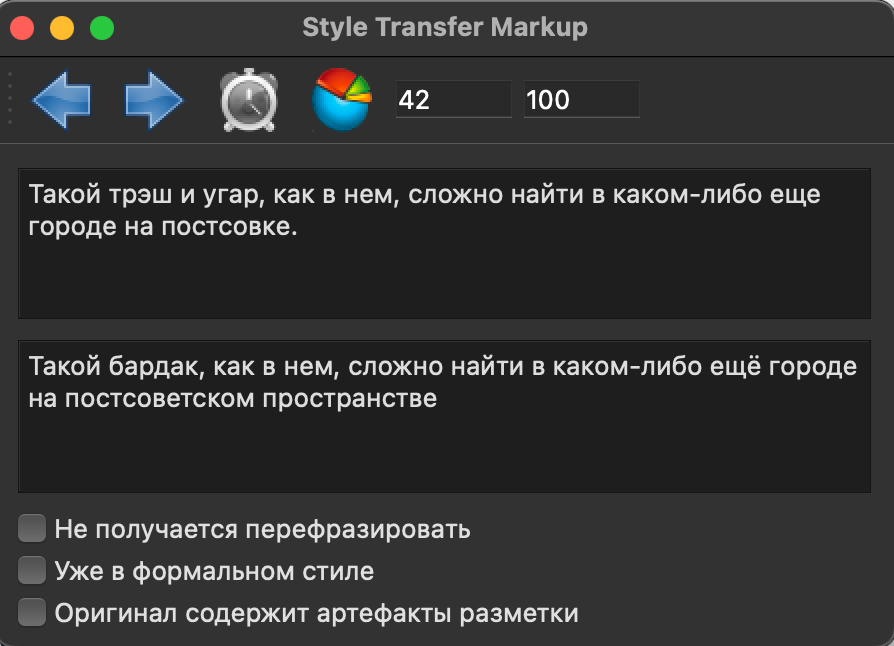
\includegraphics[width=0.8\textwidth]{figures/data_tool_rggu.png}
  \caption{Программа разметки данных для студентов РГГУ}
  \label{fig:data_tool_rggu}
\end{figure}

Вверху указано переводимое предложение, а в нижнем окне студент должен записать свой парафраз.
Так же, если предложение вызывает трудности у студента, то его можно соответствующим образом пометить.
Это сделано для того, чтобы можно было в дальнейшем фильтровать предложения.
Если оригинал содержит артефакты разметки, то можно его исправить после разметки и получить хорошее предложение. Артефакты разметки означают, что само исходное предложение качественное, но в нем остались артефакты от вики-движка и нужно вручную их почистить.


Аннотирование длилось четыре месяца и были получены следующие результаты:
\begin{itemize}
    \item Всего обработано 30118 предложений;
    \item 17881 предложение готовы к использованию;
    \item 1271 одно предложение были помечены как имеющие артефакты. После исправления артефактов и фильтрации осталось 659 предложений.
\end{itemize}
Итого получилось 18 540 предложений. Поставленная цель перевыполнена.

Студенты перевели большую часть неформальностей, интернет-мемов и отсылок, а те, которые они не понимали, искали им объяснения в интернете и пытались сделать хороший перевод.
В целом эту работу можно оценить как положительную.


Однако, некоторые аспекты можно было выполнить лучше.
Со стороны студентов: несмотря на просьбы пропускать очевидно формальные предложения, часто студенты их не игнорировали и переписывали с минимальными изменениями.
С нашей стороны необходимо было более качественно подходить к фильтрованию набора данных и инвестировать больше времени в поиск более качественного алгоритма по формированию выборки.
